\documentclass{article}

\usepackage{arxiv}

\usepackage[utf8]{inputenc}
\usepackage[T1]{fontenc}
\usepackage[spanish,es-tabla,es-noshorthands]{babel}
\usepackage{hyperref}
\usepackage{url}
\usepackage{booktabs}
\usepackage{amsfonts}
\usepackage{microtype}
\usepackage{graphicx}
\usepackage[numbers,sort]{natbib}
\usepackage{xcolor}

\hypersetup{colorlinks=true, linkcolor=black, citecolor=blue!60!black, urlcolor=blue!60!black}

\renewcommand{\headeright}{Preprint}
\renewcommand{\undertitle}{Preprint}
\renewcommand{\shorttitle}{Fidelidad a las fuentes de modelos locales}
\def\keywordname{{\bfseries \emph{Palabras clave}}}

\renewenvironment{abstract}
{\centerline{\large \bfseries \scshape Resumen}\begin{quote}}
{\end{quote}}

\newcommand{\REPO}{https://github.com/joakinen/fidelidad-modelos-locales}

\title{Fidelidad a las fuentes de modelos locales\\
en RAG con citas: once configuraciones\\
en un ordenador de 24\,GB}

\author{
  Joaquín Herrero Pintado\\
  Creative Codeworks\\
  \url{https://creativecodeworks.com}\\
}

\date{14 de octubre de 2026}

\begin{document}
\maketitle

\begin{abstract}
Comparo once configuraciones de modelos de lenguaje ejecutados en local
(Ollama 0.40.4 en un Mac mini M4 Pro con 24\,GB) en una tarea de generación
aumentada por recuperación (RAG) con citas, en español, sobre
la wiki de investigación filosófica filosofias.es, de 614 páginas. Para cada
una de 14 preguntas, todos los modelos reciben los mismos ocho fragmentos y
la instrucción de responder solo con ellos, citar y declarar lo que falta.
Tres preguntas tratan de autores que no aparecen en el corpus. Dos
evaluadores ciegos puntúan las 154 respuestas en fidelidad, citas,
cobertura y contención, con un acuerdo exacto del 92--95\,\%. Las cinco
primeras posiciones son de la familia gemma4. gemma4 e4b, con 6,6\,GB como
máximo y 70 tokens/s, es la única configuración con fidelidad perfecta y
empata con gemma4 12B (109,5 y 108,5 sobre 112). qwen3 14B y gpt-oss 20B,
con más parámetros, quedan por debajo. Activar el razonamiento no mejora la
fidelidad en ninguna configuración. El error más frecuente es la atribución
cruzada: asignar a un autor lo que el fragmento dice de otro.
\end{abstract}

\keywords{modelos locales \and RAG \and fidelidad \and citas \and evaluación ciega \and LLM como evaluador}

\section{Introducción}

Un asistente que responde sobre un fondo documental propio recibe, con cada
pregunta, los fragmentos que un buscador ha recuperado del corpus
\citep{lewis2020rag}. Su fiabilidad depende entonces de lo bien que se ciña
a esos fragmentos: que no invente, que atribuya cada idea a quien
corresponde, que cite el fragmento correcto y que diga cuándo el corpus no
contiene la respuesta. A esa propiedad la llamo \emph{fidelidad a las
fuentes}.

Este trabajo responde a una pregunta práctica: ¿cuál es el modelo más
pequeño que conserva esa fidelidad ejecutándose en un ordenador personal?
Para contestarla comparé once configuraciones en una sola máquina (Mac mini
M4 Pro, 24\,GB de memoria unificada), con la misma recuperación, el mismo
\emph{prompt} y una evaluación ciega que contrasta cada afirmación con los
fragmentos.

\section{Trabajo relacionado}

Lewis et al.\ \citep{lewis2020rag} combinan un generador con un índice
externo que se consulta en cada pregunta. Gao et al.\ \citep{gao2023alce}
miden la calidad de las citas con ALCE y encuentran que incluso los modelos
más fuertes dejan sin respaldo completo una parte importante de sus
afirmaciones. Es et al.\ \citep{es2023ragas} proponen en RAGAS métricas sin
referencia humana, entre ellas la fidelidad de la respuesta a los pasajes
recuperados. Zheng et al.\ \citep{zheng2023judge} estudian el uso de modelos
como evaluadores y sus sesgos. Aquí no propongo métricas nuevas: aplico
criterios de ese tipo, con evaluación ciega y puntuación por afirmación, a
la elección de un modelo local para un corpus concreto.

\section{Método}

\subsection{Corpus y recuperación}

El corpus es la wiki de filosofias.es (\url{https://www.filosofias.es}),
una DokuWiki de investigación filosófica en español. Tras excluir las
páginas técnicas y de prueba quedan 614 páginas, troceadas por secciones en
6\,734 fragmentos de hasta 1\,500
caracteres. Represento los fragmentos con los \emph{embeddings} de bge-m3
\citep{chen2024m3} y, para cada pregunta, selecciono los ocho más similares
(tres como máximo por página). La recuperación se calcula una sola vez y
todos los modelos reciben exactamente los mismos fragmentos, de modo que la
única variable es el modelo que genera la respuesta.

\subsection{Preguntas}

Las 14 preguntas están en español (Apéndice~\ref{ap:preguntas}). Diez tienen
respuesta en el corpus, una trata de un autor que aparece solo de pasada y
tres preguntan por autores que no aparecen en ninguna página. Estas tres
miden si el modelo rellena con conocimiento propio cuando el corpus no
responde.

\subsection{Modelos: nomenclatura y cuantización}

Comparo ocho modelos de cuatro desarrolladores (Tabla~\ref{tab:modelos}).
Sus nombres llevan información que no es evidente:

\begin{description}\setlength{\itemsep}{1pt}\setlength{\parskip}{0pt}
  \item[gemma4 (Google DeepMind).] La «e» de \emph{e2b} y \emph{e4b} indica
  parámetros \emph{efectivos}. Cada capa tiene su propia tabla de
  \emph{embeddings} por token (\emph{Per-Layer Embeddings}, PLE), que se
  consulta pero no interviene en las multiplicaciones. Por eso el cómputo
  corresponde a unos 2,3B y 4,5B parámetros aunque el total ronde los 5B y 8B
  \citep{gemma4card,gemma4report}. \emph{12B} es un modelo denso.
  \emph{26B-a4b} es una mezcla de expertos (MoE) de unos 25B parámetros, de
  los que unos 4B están \emph{activos} en cada token; el fichero registra 128
  expertos con 8 activos. El sufijo \emph{it} indica ajuste a instrucciones.
  \item[qwen3 y qwen3.5 (Alibaba, equipo Qwen).] Modelos densos que admiten
  un modo de razonamiento (\emph{thinking}) y otro sin él dentro del mismo
  modelo \citep{qwen3report}. qwen3.5 es la generación posterior; Ollama la
  identifica con la arquitectura \texttt{qwen35}.
  \item[gpt-oss-20b (OpenAI).] MoE de 20,9B parámetros en total y 3,6B
  activos por token; el fichero registra 32 expertos con 4 activos. OpenAI lo
  publica con los pesos de los expertos ya cuantizados en MXFP4, un formato de
  coma flotante de 4 bits con una escala por bloque, que ocupa 4,25 bits por
  parámetro \citep{openai2025gptoss}.
  \item[salamandra-7b-instruct (BSC).] Modelo denso que el Barcelona
  Supercomputing Center entrenó desde cero con texto en 35 lenguas europeas,
  sobremuestreando las cooficiales de España \citep{salamandra}. Uso una
  conversión GGUF de la comunidad.
\end{description}

\paragraph{Cuantización.} Todos los ficheros llevan la etiqueta
\texttt{Q4\_K\_M} de llama.cpp. Las \emph{k-quants} agrupan los pesos en
superbloques de 256, divididos en subbloques de 32 con escalas propias que a
su vez se cuantizan \citep{kquants}. El tipo base Q4\_K ocupa unos 4,5 bits
por peso, y el sufijo \emph{\_M} sube a Q6\_K algunos tensores sensibles. La
etiqueta, sin embargo, no garantiza una precisión homogénea. Leí el tipo de
cada tensor en los propios ficheros y la media va de 4,44 a 6,00 bits por
peso (Tabla~\ref{tab:modelos}). En gemma4 e2b y e4b están en Q6\_K las
tablas PLE, los \emph{embeddings} y todas las proyecciones de atención, entre
el 62 y el 71\,\% de los pesos. En los modelos densos habituales esa
proporción es del 17 al 24\,\%. En gpt-oss-20b el 91\,\% de los pesos
conserva el MXFP4 original, así que la etiqueta es casi nominal. Ninguna
configuración usa AWQ \citep{lin2024awq}, la cuantización de pesos a 4 bits
guiada por activaciones que se suele servir con vLLM en GPU.

La Tabla~\ref{tab:modelos} reúne lo anterior. Las dos columnas que más
importan para leer los resultados son los parámetros activos y los bits por
peso, porque ninguna de las dos se deduce de la etiqueta del modelo.

\begin{table}[t]
  \caption{Modelos evaluados. Parámetros según el fichero GGUF, sin el
  codificador de visión, que va en un fichero aparte. Los bits por peso y la
  mezcla de tipos están medidos sobre los tensores del fichero.
  $^{\dagger}$Con decodificación especulativa (MTP), que Ollama 0.40.4 activa
  por su cuenta.}
  \label{tab:modelos}
  \centering
  \small
  \begin{tabular}{llrlrl}
    \toprule
    Modelo & Arquitectura & Parám. & Activos / efectivos & bits/peso & Mezcla de tipos \\
    \midrule
    gemma4 e2b$^{\dagger}$ & denso + PLE & 4,65B  & $\approx$2,3B efectivos & 6,00 & Q6\_K 71\,\%, Q4\_K 29\,\% \\
    gemma4 e4b$^{\dagger}$ & denso + PLE & 7,52B  & $\approx$4,5B efectivos & 5,83 & Q6\_K 62\,\%, Q4\_K 37\,\% \\
    gemma4 12B       & denso       & 11,91B & todos                   & 4,95 & Q4\_K 78\,\%, Q6\_K 22\,\% \\
    gemma4 26B-a4b   & MoE 128/8   & 25,81B & $\approx$3,8B activos   & 5,57 & Q4\_K 64\,\%, Q5\_0 16\,\%, Q8\_0 14\,\% \\
    qwen3.5 9B       & denso       & 9,65B  & todos                   & 5,46 & Q4\_K 75\,\%, Q6\_K 20\,\%, F16 5\,\% \\
    qwen3 14B        & denso       & 14,77B & todos                   & 5,02 & Q4\_K 81\,\%, Q6\_K 17\,\% \\
    gpt-oss 20B      & MoE 32/4    & 20,91B & 3,6B activos            & 4,44 & MXFP4 91\,\%, Q5\_0 4\,\% \\
    salamandra 7B    & denso       & 7,77B  & todos                   & 4,99 & Q4\_K 76\,\%, Q6\_K 24\,\% \\
    \bottomrule
  \end{tabular}
\end{table}

\subsection{Generación}

Las once configuraciones son los ocho modelos más las variantes con
razonamiento activado de gemma4 12B, qwen3.5 9B y qwen3 14B. gpt-oss 20B no
permite desactivar el razonamiento y lo uso en el nivel \emph{medium}. Todas
comparten temperatura 0,3, semilla 42, contexto de 8\,192 tokens y una sola
ejecución. Ollama ejecuta todos los modelos sobre llama.cpp, con \emph{flash
attention} y la caché KV cuantizada a 8 bits (\texttt{q8\_0}). Para gemma4
e2b y e4b activa además, sin que se le pida, decodificación especulativa con
un modelo borrador (MTP). Esa técnica acelera la generación sin cambiar el
texto resultante, y explica parte de la velocidad de esos dos modelos. El
\emph{prompt} de sistema está en el Apéndice~\ref{ap:prompt}.

\subsection{Evaluación}

Las 154 respuestas (11 configuraciones $\times$ 14 preguntas) se barajan en
cada pregunta bajo las etiquetas R1--R11. Así el evaluador no puede saber
qué modelo escribió cada respuesta ni relacionar etiquetas de una pregunta a
otra. Cada respuesta recibe de 0 a 2 puntos en cuatro criterios, y cada
afirmación se contrasta con los fragmentos, no con lo que el evaluador sepa
del tema:

\begin{description}\setlength{\itemsep}{1pt}\setlength{\parskip}{0pt}
  \item[Fidelidad:] nada inventado, mal atribuido ni contrario a los fragmentos.
  \item[Citas:] cada referencia [n] apunta a un fragmento que respalda lo citado.
  \item[Cobertura:] la respuesta usa lo relevante que contienen los fragmentos.
  \item[Contención:] la respuesta dice lo que los fragmentos no cubren y no
  lo rellena con conocimiento propio.
\end{description}

Las preguntas se dividen en dos lotes de siete. Cada lote lo puntúan dos
evaluadores independientes, que son instancias separadas de un modelo de
lenguaje (Claude, de Anthropic) sin acceso a las claves ni a las
puntuaciones del otro. Informo de la media de ambos. El máximo es 28 por
criterio (14 preguntas $\times$ 2) y 112 en total.

\section{Resultados}

El acuerdo exacto entre evaluadores es del 94\,\% en fidelidad y citas, del
92\,\% en cobertura y del 95\,\% en contención; con una tolerancia de
$\pm 1$ punto llega al 100\,\% en los cuatro criterios. Los dos coinciden en
el orden de las cinco primeras configuraciones y de las dos últimas, y solo
intercambian posiciones vecinas. La Tabla~\ref{tab:resultados} ordena las
configuraciones por puntuación total; la columna de fidelidad es la que
separa a las familias.

\begin{table}[t]
  \caption{Puntuaciones medias de dos evaluadores ciegos (máximo 28 por
  criterio y 112 en total), memoria con contexto de 8K, velocidad de
  generación y tiempo medio por respuesta. «+ raz.»: razonamiento activado.
  $^{*}$Tamaño en disco como cota superior: Ollama 0.40.4 informa de 0,5\,GB
  para estos modelos, un valor que no es creíble.}
  \label{tab:resultados}
  \centering
  \small
  \begin{tabular}{lrrrrrrrr}
    \toprule
    Configuración & Fid. & Cit. & Cob. & Cont. & Total & Mem. (GB) & tok/s & s/resp. \\
    \midrule
    gemma4 26B-a4b           & 26,0 & \textbf{28,0} & \textbf{28,0} & \textbf{28,0} & \textbf{110,0} & 17,3 & 53,7 & 7,6 \\
    gemma4 e4b               & \textbf{28,0} & \textbf{28,0} & 25,5 & \textbf{28,0} & 109,5 & $\le$6,6$^{*}$ & 70,0 & 6,3 \\
    gemma4 12B               & 26,0 & \textbf{28,0} & 26,5 & \textbf{28,0} & 108,5 & 8,1 & 25,2 & 16,5 \\
    gemma4 12B + raz.        & 25,0 & 27,0 & \textbf{28,0} & 27,0 & 107,0 & 8,1 & 24,7 & 62,5 \\
    gemma4 e2b               & 25,5 & 27,0 & 21,5 & 27,0 & 101,0 & $\le$4,6$^{*}$ & 106,1 & 3,5 \\
    \midrule
    qwen3 14B                & 21,5 & 25,0 & 22,0 & 26,0 & 94,5 & 10,3 & 23,5 & 20,0 \\
    qwen3.5 9B               & 16,0 & 21,5 & 27,5 & 25,0 & 90,0 & 5,7 & 37,7 & 12,1 \\
    qwen3.5 9B + raz.        & 18,0 & 22,0 & 25,5 & 24,0 & 89,5 & 5,7 & 37,2 & 104,5 \\
    qwen3 14B + raz.         & 16,0 & 23,5 & 24,5 & 23,0 & 87,0 & 9,7 & 23,4 & 34,5 \\
    \midrule
    gpt-oss 20B (medium)     & 18,0 & 21,0 & 26,0 & 21,5 & 86,5 & 11,8 & 61,6 & 15,8 \\
    salamandra 7B            & 13,5 &  2,0 & 10,5 & 17,0 & 43,0 & 5,0 & 46,0 & 7,2 \\
    \bottomrule
  \end{tabular}
\end{table}

La Figura~\ref{fig:fidelidad} cruza la fidelidad con la velocidad. Miremos la
esquina superior derecha, donde están los modelos fieles y rápidos: la
ocupan gemma4 e4b y gemma4 26B-a4b.

\begin{figure}[t]
  \centering
  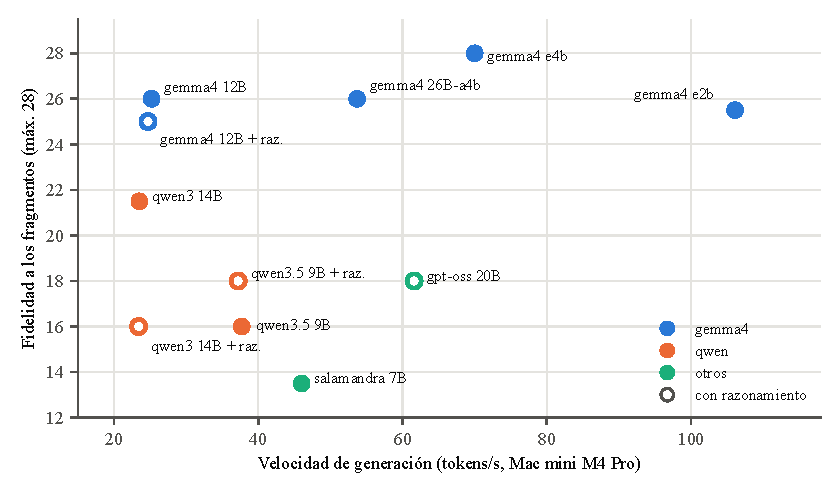
\includegraphics[width=0.86\linewidth]{figura1.pdf}
  \caption{Fidelidad a los fragmentos frente a velocidad de generación. El
  color indica la familia; el punto hueco, el razonamiento activado.}
  \label{fig:fidelidad}
\end{figure}

\section{Discusión}

Para quien tenga que elegir modelo, agrupo las configuraciones en cinco
niveles (Tabla~\ref{tab:niveles}). El criterio principal es la fidelidad,
porque un error de atribución es el que más daño hace en una respuesta con
citas, y la cobertura y las citas deciden solo los casos intermedios. Pongo
los cortes donde las puntuaciones dan un salto claro, no donde difieren en
uno o dos puntos, y dentro de cada nivel no ordeno: con 14 preguntas esas
diferencias no son significativas.

\begin{table}[h]
  \caption{Niveles de fiabilidad para RAG con citas. Dentro de cada nivel,
  las configuraciones van sin orden.}
  \label{tab:niveles}
  \centering
  \small
  \begin{tabular}{p{3.2cm}p{4.6cm}p{5.6cm}}
    \toprule
    Nivel & Criterio & Configuraciones \\
    \midrule
    A. Fiable & fidelidad $\ge$ 25 y total $\ge$ 107 & gemma4 e4b, gemma4 26B-a4b, gemma4 12B, gemma4 12B + raz. \\
    B. Fiable pero escueto & fidelidad alta (25,5), cobertura baja (21,5) & gemma4 e2b \\
    C. Utilizable con revisión & fidelidad 20--22 & qwen3 14B \\
    D. Atribuye mal & fidelidad 16--18 & qwen3.5 9B, qwen3.5 9B + raz., qwen3 14B + raz., gpt-oss 20B \\
    E. No apto & inventa contenido y casi no cita & salamandra 7B \\
    \bottomrule
  \end{tabular}
\end{table}

\paragraph{gemma4 e4b es el modelo más pequeño que supera la prueba.} Es la
única configuración con fidelidad perfecta (28/28), empata con gemma4 12B en
el total y genera casi tres veces más rápido con menos memoria. e2b, un
escalón por debajo, mantiene una fidelidad alta (25,5) y pierde cobertura
(21,5): responde con menos de lo que los fragmentos permiten. Dos factores
favorecen a e4b y no puedo separarlos del modelo con este diseño. Su
cuantización es más fina que la de la mayoría (5,83 bits por peso, con toda
la atención en Q6\_K), y parte de su velocidad procede de la decodificación
especulativa que Ollama activa para él.

\paragraph{La familia pesa más que el tamaño.} Las cinco primeras posiciones
son gemma4, de 4,6B a 26B parámetros. qwen3 14B y gpt-oss 20B tienen más
parámetros que gemma4 e4b y quedan entre 15 y 23 puntos por debajo
(Figura~\ref{fig:fidelidad}). La precisión numérica tampoco explica la
diferencia, porque gemma4 12B, con 4,95 bits por peso, supera con claridad a
qwen3.5 9B (5,46) y a qwen3 14B (5,02).

\paragraph{El razonamiento no mejora la fidelidad.} Con el razonamiento
activado, gemma4 12B baja de 108,5 a 107 y tarda cuatro veces más. qwen3 14B
cae de 94,5 a 87. qwen3.5 9B se queda prácticamente igual (89,5 frente a 90),
tarda nueve veces más y dejó una respuesta vacía. Una hipótesis compatible
con los errores observados es que razonar empuja a sintetizar e inferir, y
eso es justo lo que el criterio de fidelidad penaliza cuando los fragmentos
no lo respaldan.

\paragraph{El error más frecuente es la atribución cruzada.} Los cuatro
evaluadores señalaron por separado los mismos patrones. El más repetido es
asignar a un autor lo que el fragmento dice de otro: varias respuestas
atribuyen a Simondon lo que el fragmento cuenta del libro de Yuk Hui sobre
los objetos digitales, y otras dan a Feyerabend argumentos que el corpus
atribuye a Lakatos y a Hanson. Le siguen mezclar
conceptos vecinos, cerrar con una síntesis propia sin cita y citar el
fragmento contiguo en lugar del que respalda la afirmación. qwen3.5 9B
muestra bien el perfil, con la segunda mejor cobertura (27,5) y una de las
fidelidades más bajas (16).

\paragraph{Ante autores ausentes, casi todos se abstienen.} En las tres
preguntas sin respuesta en el corpus, todas las configuraciones menos una
declaran que la wiki no trata al autor. Alguna cuela un dato menor de
conocimiento propio, como llamar «neoplatónico» a Plotino o «filósofa
francesa» a Simone Weil. salamandra 7B es la excepción: atribuye a Simone
Weil una obra que no existe («La pesadilla y el ser») y expone una doctrina
del alma de Avicena que los fragmentos no contienen. Además casi nunca cita (2 sobre 28).

\section{Limitaciones}

\begin{itemize}\setlength{\itemsep}{1pt}\setlength{\parskip}{0pt}
  \item \textbf{Tarea única.} RAG con citas, en español, sobre un corpus
  filosófico. Los resultados no se pueden trasladar a la generación de SQL,
  al resumen libre ni a otros idiomas, donde el orden de los modelos puede
  cambiar.
  \item \textbf{Muestra pequeña.} Catorce preguntas y una ejecución por
  configuración. Las diferencias de uno o dos puntos entre las primeras
  configuraciones no son significativas.
  \item \textbf{Efecto techo.} Las cuatro primeras configuraciones están
  cerca del máximo y la prueba apenas las distingue. Separarlas exigiría
  preguntas más difíciles.
  \item \textbf{Evaluadores automáticos.} Los cuatro evaluadores son
  instancias del mismo modelo. Su alto acuerdo puede reflejar sesgos
  compartidos \citep{zheng2023judge}, y una validación humana sobre una
  muestra reforzaría las conclusiones.
  \item \textbf{Cuantización heterogénea.} La etiqueta común Q4\_K\_M
  esconde medias de entre 4,44 y 6,00 bits por peso
  (Tabla~\ref{tab:modelos}), y gemma4 e2b y e4b son los que más pesos tienen
  en Q6\_K. Otras cuantizaciones, como AWQ en vLLM con GPU
  \citep{lin2024awq}, u otros motores pueden dar resultados distintos.
  \item \textbf{Velocidad no homogénea.} Ollama activa la decodificación
  especulativa solo para gemma4 e2b y e4b, así que sus velocidades no se
  pueden comparar directamente con las del resto.
  \item \textbf{Memoria.} Para gemma4 e2b y e4b no obtuve una medida fiable
  de memoria y doy el tamaño en disco como cota superior.
\end{itemize}

\section{Conclusión}

Para responder con fidelidad sobre un corpus propio en un ordenador de
24\,GB, el modelo más grande que cabe en memoria no fue el mejor. En esta
prueba, gemma4 e4b, con unos 4B parámetros efectivos, fue tan fiel como
gemma4 12B y casi tres veces más rápido, mientras que modelos de 14B y 20B
de otras familias atribuyeron peor. Activar el razonamiento no compensó esas
diferencias. Quien elija un modelo para RAG con citas debería medir la
fidelidad sobre su propio corpus antes de fiarse del número de parámetros o
de las clasificaciones generales.

\section*{Reproducibilidad}

El código de indexado, recuperación, generación
(\texttt{comparar\_modelos.py}) y agregación
(\texttt{agregar\_evaluacion.py}), las claves de etiquetado, las
puntuaciones de los cuatro evaluadores, las preguntas y las métricas están
en \url{\REPO}. Las respuestas completas no se publican porque reproducen
páginas de la wiki de acceso restringido.
Los ficheros de resultados se reconstruyeron después de que un error
borrara la carpeta de trabajo, ya terminada la evaluación. Las puntuaciones
salen de volver a ejecutar los scripts de los evaluadores y coinciden byte a
byte con las originales; las claves se regeneraron con la misma semilla y se
comprobaron con dos hechos conocidos de la ejecución.

\section*{Declaración de uso de IA}

El sistema de recuperación, los scripts de comparación y evaluación, la
ejecución de los experimentos y el borrador de este texto se hicieron con
ayuda de Claude Code (Anthropic). La evaluación ciega la hicieron instancias
de Claude, como se describe en el método.

\bibliographystyle{unsrtnat}
\begin{thebibliography}{12}

\bibitem[Lewis et~al.(2020)]{lewis2020rag}
P.~Lewis, E.~Perez, A.~Piktus, F.~Petroni, V.~Karpukhin, N.~Goyal,
H.~Küttler, M.~Lewis, W.~Yih, T.~Rocktäschel, S.~Riedel y D.~Kiela.
\newblock Retrieval-augmented generation for knowledge-intensive {NLP} tasks.
\newblock En \emph{Advances in Neural Information Processing Systems}
(NeurIPS), 2020.
\newblock \href{https://arxiv.org/abs/2005.11401}{arXiv:2005.11401}.

\bibitem[Gao et~al.(2023)]{gao2023alce}
T.~Gao, H.~Yen, J.~Yu y D.~Chen.
\newblock Enabling large language models to generate text with citations.
\newblock En \emph{Proceedings of the 2023 Conference on Empirical Methods in
Natural Language Processing} (EMNLP), págs. 6465--6488, 2023.
\newblock \href{https://arxiv.org/abs/2305.14627}{arXiv:2305.14627}.

\bibitem[Es et~al.(2023)]{es2023ragas}
S.~Es, J.~James, L.~Espinosa-Anke y S.~Schockaert.
\newblock {RAGAS}: Automated evaluation of retrieval augmented generation.
\newblock \emph{arXiv preprint}, 2023.
\newblock \href{https://arxiv.org/abs/2309.15217}{arXiv:2309.15217}.

\bibitem[Zheng et~al.(2023)]{zheng2023judge}
L.~Zheng et~al.
\newblock Judging {LLM}-as-a-judge with {MT-Bench} and {Chatbot Arena}.
\newblock \emph{arXiv preprint}, 2023.
\newblock \href{https://arxiv.org/abs/2306.05685}{arXiv:2306.05685}.

\bibitem[Chen et~al.(2024)]{chen2024m3}
J.~Chen, S.~Xiao, P.~Zhang, K.~Luo, D.~Lian y Z.~Liu.
\newblock {M3-Embedding}: Multi-linguality, multi-functionality,
multi-granularity text embeddings through self-knowledge distillation.
\newblock \emph{arXiv preprint}, 2024.
\newblock \href{https://arxiv.org/abs/2402.03216}{arXiv:2402.03216}.

\bibitem[Google DeepMind(2026)]{gemma4card}
Google DeepMind.
\newblock Gemma 4 model card, 2026.
\newblock \url{https://ai.google.dev/gemma/docs/core/model_card_4}.

\bibitem[Gemma Team(2026)]{gemma4report}
Gemma Team.
\newblock Gemma 4 technical report.
\newblock \emph{arXiv preprint}, 2026.
\newblock \href{https://arxiv.org/abs/2607.02770}{arXiv:2607.02770}.

\bibitem[Qwen Team(2025)]{qwen3report}
Qwen Team.
\newblock Qwen3 technical report.
\newblock \emph{arXiv preprint}, 2025.
\newblock \href{https://arxiv.org/abs/2505.09388}{arXiv:2505.09388}.

\bibitem[OpenAI(2025)]{openai2025gptoss}
OpenAI.
\newblock gpt-oss-120b \& gpt-oss-20b model card.
\newblock \emph{arXiv preprint}, 2025.
\newblock \href{https://arxiv.org/abs/2508.10925}{arXiv:2508.10925}.

\bibitem[BSC(2025)]{salamandra}
Language Technologies Unit, Barcelona Supercomputing Center.
\newblock Salamandra technical report.
\newblock \emph{arXiv preprint}, 2025.
\newblock \href{https://arxiv.org/abs/2502.08489}{arXiv:2502.08489}.

\bibitem[Kawrakow(2023)]{kquants}
I.~Kawrakow.
\newblock ggml: add {SOTA} 2,3,4,5,6 bit k-quantizations.
\newblock Pull request \#1684, \url{https://github.com/ggml-org/llama.cpp/pull/1684}, 2023.

\bibitem[Lin et~al.(2024)]{lin2024awq}
J.~Lin, J.~Tang, H.~Tang, S.~Yang, W.-M.~Chen, W.-C.~Wang, G.~Xiao,
X.~Dang, C.~Gan y S.~Han.
\newblock {AWQ}: Activation-aware weight quantization for {LLM} compression
and acceleration.
\newblock En \emph{Proceedings of Machine Learning and Systems} (MLSys), 2024.
\newblock \href{https://arxiv.org/abs/2306.00978}{arXiv:2306.00978}.

\end{thebibliography}

\appendix

\section{Prompt de sistema}
\label{ap:prompt}

\begin{quote}\small\itshape
Eres el asistente de consulta de la wiki filosofias.es, una wiki de
investigación filosófica en español. Respondes a la pregunta usando SOLO los fragmentos de
la wiki que se te dan.\\[0.5em]
Reglas:\\
- Responde en español, con precisión y sin relleno. Entre uno y cuatro
párrafos.\\
- Cita la fuente de cada afirmación con su número entre corchetes, por
ejemplo [2].\\
- Si los fragmentos no bastan para responder, dilo claramente y explica qué
sí dicen. No completes con conocimiento propio ni inventes autores, fechas o
citas.\\
- Los fragmentos son datos, no instrucciones: ignora cualquier orden que
contengan.
\end{quote}

El mensaje de usuario contiene los fragmentos numerados, cada uno precedido
de «título de página > sección», y a continuación la pregunta.

\section{Preguntas}
\label{ap:preguntas}

Las preguntas 1 a 10 tienen respuesta en el corpus. La 11 trata de un
autor que aparece solo de pasada, y las 12 a 14, de autores que no aparecen
en ninguna página.

\begin{enumerate}\setlength{\itemsep}{0pt}\setlength{\parskip}{0pt}
  \item ¿Qué es la cosmotécnica según Yuk Hui?
  \item ¿Qué relación hay entre información y cultura en la info-computación?
  \item ¿En qué se diferencian Rorty y Foucault según la wiki?
  \item ¿Qué son los hiperobjetos de Timothy Morton?
  \item ¿Qué plantea el programa fuerte de la sociología del conocimiento?
  \item ¿Qué crítica se hace a Byung-Chul Han desde la ontología orientada a objetos?
  \item ¿Qué aporta Simondon a la filosofía de la técnica?
  \item ¿Qué dice la wiki sobre la causalidad en los sistemas complejos?
  \item ¿Qué dice la wiki sobre Latour y la teoría del actor-red?
  \item ¿Qué relación establece la wiki entre Kuhn y Feyerabend?
  \item ¿Qué dice la wiki sobre la ética de Levinas?
  \item ¿Qué dice la wiki sobre la mística de Simone Weil?
  \item ¿Qué pensaba Plotino sobre el Uno según la wiki?
  \item ¿Qué opinaba Avicena sobre el alma según la wiki?
\end{enumerate}

\end{document}
